
\documentclass [PhD] {uclathes}

\usepackage{graphicx}
\graphicspath{ {./figures/} }
\usepackage{cite}
\usepackage[colorlinks]{hyperref}
\hypersetup{
     colorlinks = true,
     linkcolor = blue,
     anchorcolor = blue,
     citecolor = blue,
     filecolor = blue,
     urlcolor = blue
}


% \input {mymacros}                         % personal LaTeX macros

%%%%%%%%%%%%%%%%%%%%%%%%%%%%%%%%%%%%%%%%%%%%%%%%%%%%%%%%%%%%%%%%%%%%%%
%
% Usually things live in separate flies.
%
% \input {prelim}                           % preliminary page info

%%%%%%%%%%%%%%%%%%%%%%%%%%%%%%%%%%%%%%%%%%%%%%%%%%%%%%%%%%%%%%%%%%%%%%%%
%                                                                      %
%                          PRELIMINARY PAGES                           %
%                                                                      %
%%%%%%%%%%%%%%%%%%%%%%%%%%%%%%%%%%%%%%%%%%%%%%%%%%%%%%%%%%%%%%%%%%%%%%%%

\title          {Discovering Data-Driven Actionable Intelligence\\
for Clinical Decision Support}
\author         {Ahmed M. Alaa H. H. Ibrahim}
\department     {Electrical and Computer Engineering}
% Note:  degreeyear should be optional, but as of  5-Feb-96
% it seems required or you get a year of ``2''.   -johnh
\degreeyear     {2019}

%%%%%%%%%%%%%%%%%%%%%%%%%%%%%%%%%%%%%%%%%%%%%%%%%%%%%%%%%%%%%%%%%%%%%%%%

\chair          {Mihaela van der Schaar}
\member         {Douglas Bell}
\member         {Patricia Ganz}
\member         {Yahya Rahmat-Samii}
\member         {Greg Pottie}



%%%%%%%%%%%%%%%%%%%%%%%%%%%%%%%%%%%%%%%%%%%%%%%%%%%%%%%%%%%%%%%%%%%%%%%%

\dedication     {\textsl{To my parents and my brothers.}}

%%%%%%%%%%%%%%%%%%%%%%%%%%%%%%%%%%%%%%%%%%%%%%%%%%%%%%%%%%%%%%%%%%%%%%%%

\acknowledgments {
I would not have been able to complete this dissertation without the help and support
of my family, my adviser, my colleagues and friends. I am deeply grateful.

First, I wish to thank my adviser, Professor Mihaela van der Schaar, for her kindness~and unyielding support. This dissertation would not have been possible without her~research~vision. Her new ideas, insights, opportunities and willingness to intrepidly explore multidisciplinary research terrains have had a profound impact on my development as a researcher. I am deeply grateful for her invaluable support and immense help. Thank you for everything, Mihaela. I also thank the other members of my dissertation committee, Professor Greg Pottie, Professor Yahya Rahmat-Samii, Professor Patricia Ganz, and Dr. Douglas Bell for their valuable perspectives and thoughtful feedback. 

I would also like to thank all of my co-authors and collaborators at UCLA; Jinsung Yoon, Scott Hu, William Zame, Changhee Lee, Kartik Ahuja, William Hsu, Kyeong Moon and Martin Cadeiras. It has been a great privilege to be able to work with such talented people. I have also been fortunate to enjoy the collegiality of my labmates; Onur Atan, Trent Kyono, William Whoiles, Yangbo Song, Simpson Zhang, Jie Xu and Yuanzhang Xiao, with whom I had many insightful research discussions. I would also like to thank my friends at UCLA for their companionship and support. I especially want to thank Ahmed Hareedy, Mohammed Karmoose, Yahya Ezzeldin, Omar Hussien, Moustafa Alzantot, and Safa Cicek. 

I have been so lucky to spend some time on the other side of the Atlantic as a visiting student at Oxford University. There, I was fortunate to work with my colleagues at Oxford University, Ioana Bica, James Jordon, Bryan Lim, and Michael Weisz, and my colleagues at Cambridge University, Yao Zhang, Zhaozhi Qian, Alexis Bellot, and Daniel Jarrett.     

During my visit in the UK, I was blessed to be able to collaborate with many clinicians who provided me with the clinical data, guidance and feedback that made the clinical application of my work come to life. I would like to especially thank Dr. Jem~Rashbass~(National~Director for Disease Registration at Public Health England) for granting me access to the UK breast cancer registry data, and Dr Janet Allen (Director of Strategic Innovation at the UK Cystic Fibrosis Trust) for enabling my access to the UK Cystic Fibrosis registry. I would also like to thank my clinical collaborators at Cambridge University, Andres Floto, Fiona Gilbert, Emanuele Di Angelantonio, James Rudd, and my collaborator at Queen Mary University of London, Deepti Gurdasani.  

Finally, and most importantly, I wish to thank my parents, Hadeel and Alaa, and my borthers, Ali and Sherif for their love and support. No words can express what your encouragement and support have meant to me. 
}

%%%%%%%%%%%%%%%%%%%%%%%%%%%%%%%%%%%%%%%%%%%%%%%%%%%%%%%%%%%%%%%%%%%%%%%%

\vitaitem   {2011}
                {Bachelor in Communications and Computer Engineering,\\ 
                Cairo University, Cairo, Egypt}
\vitaitem   {2011--2014}
                {Teaching Assistant, Communications Engineering Department,\\ Cairo University, Cairo, Egypt}
\vitaitem   {2014}
                {Master of Science in Electronics and Communications Engineering,\\
Cairo University, Cairo, Egypt}
\vitaitem   {2014}
                {Graduate Division Fellowship, Electrical Engineering,\\ University of California, Los Angeles.}
\vitaitem   {2014--2019}
                {Research Assistant,\\ University of California, Los Angeles.}
\vitaitem   {2017--2018}
                {Recognized PhD Student,\\ University of Oxford, United Kingdom.}

%%%%%%%%%%%%%%%%%%%%%%%%%%%%%%%%%%%%%%%%%%%%%%%%%%%%%%%%%%%%%%%%%%%%%%%%

\publication {\textbf{A. M. Alaa}, T. Bolton, E. Di Angelantonio, J. H. F. Rudd, M. van der Schaar, ``Cardiovascular Disease Risk Prediction using Automated Machine Learning: A Prospective Study of 423,604 UK Biobank Participants,'' \textit{PloS One}, 2019.

\vspace{-.15in}
\hspace{-.3in}
\textbf{A. M. Alaa}, M. van der Schaar, ``Demystifying Black-box Models with Symbolic Metamodels,'' \textit{Neural Information Processing Systems} (NeurIPS), 2019.

\vspace{-.15in}
\hspace{-.3in}
\textbf{A. M. Alaa}, M. van der Schaar, ``Attentive State-Space Modeling of Disease Progression,'' \textit{Neural Information Processing Systems} (NeurIPS), 2019.

\vspace{-.15in}
\hspace{-.3in}
\textbf{A. M. Alaa}, M. van der Schaar, ``Validating Causal Inference Models via Influence Functions,'' \textit{International Conference on Machine Learning} (ICML), 2019.

\vspace{-.15in}
\hspace{-.3in}
I. Bica, \textbf{A. M. Alaa}, M. van der Schaar, ``Estimating Counterfactual Treatment Outcomes over Time through Adversarially Balanced Representations,'' \textit{NeurIPS Machine Learning for Health Workshop}, 2019.

\vspace{-.15in}
\hspace{-.3in}
I. Bica, \textbf{A. M. Alaa}, M. van der Schaar, ``Time Series Deconfounder: Estimating Treatment Effects over Time in the Presence of Hidden Confounders,'' \textit{NeurIPS Machine Learning for Health Workshop}, 2019.

\vspace{-.15in}
\hspace{-.3in}
C. Lee, W. R. Zame, \textbf{A. M. Alaa}, M. van der Schaar, ``Temporal Quilting for Survival Analysis,'' \textit{International Conference on Artificial Intelligence and Statistics} (AISTATS), 2019.

\vspace{-.15in}
\hspace{-.3in}
\textbf{A. M. Alaa}, M. van der Schaar, ``Prognostication and Risk Factors for Cystic Fibrosis via Automated Machine Learning,'' \textit{Scientific Reports}, 2018.

\vspace{-.15in}
\hspace{-.3in}
\textbf{A. M. Alaa}, M. van der Schaar, ``Bayesian Nonparametric Causal Inference: Information Rates \& Learning Algorithms,'' \textit{IEEE Journal of Selected Topics in Signal Processing}, 2018.

\vspace{-.15in}
\hspace{-.3in}
J. Yoon, W. R. Zame, A. Banerjee, M. Cadeiras, \textbf{A. M. Alaa}, M. van der Schaar, ``Personalized survival predictions via Trees of Predictors: An application to cardiac transplantation,'' \textit{PloS One}, 2018.

\vspace{-.15in}
\hspace{-.3in}
B. Lim, \textbf{A. M. Alaa}, M. van der Schaar, ``Forecasting Treatment Responses Over Time Using Recurrent Marginal Structural Networks,'' \textit{Neural Information Processing Systems} (NeurIPS), 2018.

\vspace{-.15in}
\hspace{-.3in}
\textbf{A. M. Alaa}, M. van der Schaar, ``AutoPrognosis: Automated Clinical Prognostic Modeling via Bayesian Optimization with Structured Kernel Learning,'' \textit{International Conference on Machine Learning} (ICML), 2018.

\vspace{-.15in}
\hspace{-.3in}
\textbf{A. M. Alaa}, M. van der Schaar, ``Limits of Estimating Heterogeneous Treatment Effects: Guidelines for Practical Algorithm Design,'' \textit{International Conference on Machine Learning} (ICML), 2018.

\vspace{-.15in}
\hspace{-.3in}
\textbf{A. M. Alaa}, T. Daniels, R. Floto, M. van der Schaar, ``Machine Learning-Based Predictions of Prognosis in Cystic Fibrosis,'' \textit{Pediatric Pulmonology}, 2018. \textbf{(Abstract)}

\vspace{-.15in}
\hspace{-.3in}
\textbf{A. M. Alaa}, T. Bolton, E. Di Angelantonio, J. Rudd, M. van der Schaar, ``Cardiovascular Disease Risk Prediction Using Machine Learning: A Prospective Cohort Study of 423,604 Participants,'' \textit{Circulation}, 2018. \textbf{(Abstract)}

\vspace{-.15in}
\hspace{-.3in} 
A. Banerjee, J. Yoon, W. R. Zame, M. Cadeiras, \textbf{A. M. Alaa}, M. van der Schaar, ``Personalized risk prediction for wait-list and post-transplant mortality in cardiac transplantation: machine learning using predictive clusters,'' \textit{European Heart Journal}, 2017. \textbf{(Abstract)}

\vspace{-.15in}
\hspace{-.3in}
\textbf{A. M. Alaa}, M. van der Schaar, ``A Hidden Absorbing Semi-Markov Model for Informatively Censored Temporal Data,'' \textit{Journal of Machine Learning Research}, 2017.

\vspace{-.15in}
\hspace{-.3in}
\textbf{A. M. Alaa}, J. Yoon, S. Hu, and M. van der Schaar, ``Personalized Risk Scoring for Critical Care Prognosis using Mixtures of Gaussian Processes,'' \textit{IEEE Transactions on Biomedical Engineering}, 2017.

\vspace{-.15in}
\hspace{-.3in}
\textbf{A. M. Alaa}, M. van der Schaar, ``Deep Multi-task Gaussian Processes for Survival Analysis with Competing Risks,'' \textit{Neural Information Processing Systems} (NeurIPS), 2017. \textbf{(Selected for a spotlight presentation)}

\vspace{-.15in}
\hspace{-.3in}
\textbf{A. M. Alaa}, M. van der Schaar, ``Bayesian Inference of Individualized Treatment Effects using Multi-task Gaussian Processes,'' \textit{Neural Information Processing Systems} (NeurIPS), 2017.

\vspace{-.15in}
\hspace{-.3in}
\textbf{A. M. Alaa}, M. Weisz, M. van der Schaar, ``Deep Counterfactual Networks with Propensity-Dropout,'' \textit{ICML Workshop on Principled Approaches to Deep Learning}, 2017.

\vspace{-.15in}
\hspace{-.3in}
\textbf{A. M. Alaa}, M. van der Schaar, ``Learning from Clinical Judgments: Semi-Markov-Modulated Marked Hawkes Processes for Risk Prognosis,'' \textit{International Conference on Machine Learning} (ICML), 2017.

\vspace{-.15in}
\hspace{-.3in}
\textbf{A. M. Alaa}, M. van der Schaar, ``Individualized Risk Prognosis for Critical Care Patients: A Multi-task Gaussian Process Model,'' \textit{Big Data in Medicine: Tools, Transformation and Translation, Cambridge}, 2017.

\vspace{-.15in}
\hspace{-.3in}
A. Banerjee, J. Yoon, W. R. Zame, M. Cadeiras, \textbf{A. M. Alaa}, M. van der Schaar, ``Personalized Risk Prediction using Predictive Pursuit Machine Learning: A Pilot Study in Cardiac Transplantation,'' \textit{European Society of Cardiology Congress}, 2017. \textbf{(Selected as Best Poster in Advanced Heart Failure)}

\vspace{-.15in}
\hspace{-.3in}
\textbf{A. M. Alaa}, K. Ahuja, and M. van der Schaar, ``A Micro-foundation of Social Capital in Evolving Social Networks,'' \textit{IEEE Transactions on Network Science and Engineering}, 2017.

\vspace{-.15in}
\hspace{-.3in}
\textbf{A. M. Alaa}, M. van der Schaar, ``Balancing Suspense and Surprise: Timely Decision Making with Endogenous Information Acquisition,'' \textit{Neural Information Processing Systems} (NeurIPS), 2016.

\vspace{-.15in}
\hspace{-.3in}
\textbf{A. M. Alaa}, M. van der Schaar, ``A Semi-Markov Switching Linear Gaussian Model for Censored Physiological Data,'' \textit{NeurIPS workshop on Machine Learning for Health}, 2016.

\vspace{-.15in}
\hspace{-.3in}
\textbf{A. M. Alaa}, K. H. Moon, W. Hsu and M. van der Schaar, ``ConfidentCare: A Clinical Decision Support System for Personalized Breast Cancer Screening,'' \textit{IEEE Transactions on Multimedia --- Special Issue on Multimedia-based Healthcare}, 2016.

\vspace{-.15in}
\hspace{-.3in}
\textbf{A. M. Alaa}, M. van der Schaar, ``ForecastICU: A Prognostic Decision Support System for Timely Prediction of Intensive Care Unit Admission,'' \textit{International Conference on Machine Learning} (ICML), 2016.

\vspace{-.15in}
\hspace{-.3in}
\textbf{A. M. Alaa}, J. Yoon, M. van der Schaar, ``Personalized Risk Scoring for Critical Care Patients using Mixtures of Gaussian Process Experts,'' \textit{ICML Workshop on Computational Frameworks for Personalization}, 2016.

\vspace{-.15in}
\hspace{-.3in}
\textbf{A. M. Alaa}, K. Ahuja, M. van der Schaar, " Self-organizing Networks of Information Gathering Cognitive Agents," \textit{IEEE Transactions on Cognitive Communications and Networking - Inaugural issue (invited paper)}, 2015.

}


%%%%%%%%%%%%%%%%%%%%%%%%%%%%%%%%%%%%%%%%%%%%%%%%%%%%%%%%%%%%%%%%%%%%%%%%
\abstract{The rapid digitization of healthcare has led to a proliferation of clinical data, manifesting through electronic health records, biorepositories, and disease registries. This dissertation addresses the question of how machine learning (ML) techniques can capitalize on these data resources to assist clinicians in predicting, preventing~and~treating~illness. To this end, we develop a set of ML-based, data-driven models of patient outcomes that we envision to be embedded within systems of decision support deployed at different stages of patient care. 

We focus on two broad setups for analyzing clinical data: (1) the \textit{cross-sectional} setup wherein data is collected by observing many patients at a particular point of time, and (2) the \textit{longitudinal} setup in which repeated observations of the same patient are collected over time. In both setups, we develop models that are: (a) capable of answering \textit{counter-factual} questions, i.e., can predict outcomes under alternative treatment scenarios, (b) \textit{interpretable} in the sense that clinicians can understand how the model predictions for individual patients are issued, and (c) \textit{automated} in the sense that they adaptively tune their modeling choices for the dataset at hand, with little or no need for expert intervention. Models satisfying these \textit{three} requirements would enable the realization of actionable, transparent and automated decision support systems that operate symbiotically within existing clinical workflows.

Our technical contributions are multi-faceted. In the cross-sectional data setup, we develop ML models that fulfill the aforementioned requirements (a)-(c) as follows. We start by developing a comprehensive theoretical framework for causal inference, whereby we quantify the limits to how well ML models can recover the causal effects of counter-factual treatment decisions on individual patients using observational (retrospective) data, and we build ML models --- based on \textit{Gaussian processes} --- that achieve these limits. Next, we develop a novel \textit{symbolic meta-modeling} approach for interpreting the predictions of any ML-based prognostic model by converting the ``black-box'' model into an understandable symbolic equation that relates patients' features to their predicted outcomes. Finally, we develop a model selection approach based on \textit{Bayesian optimization} that enables the automation of predictive and causal modeling. In the longitudinal data setup, we develop a novel deep probabilistic model for sequential clinical data that satisfies requirements (a)-(c) by capitalizing on the strengths of both state-space models and deep recurrent neural networks.

To demonstrate the utility of our models, we evaluate their performance on various real-world datasets for cohorts of breast cancer, cardiovascular disease and cystic fibrosis patients. We show that, compared to existing clinical scorers, our ML-based models can improve the accuracy of predicting individual-level prognoses, guide treatment decisions for individual patients, and provide insights into underlying disease mechanisms.} 

\begin {document}
\makeintropages

%%%%%%%%%%%%%%%%%%%%%%%%%%%%%%%%%%%%%%%%%%%%%%%%%%%%%%%%%%%%%%%%%%%%%%
%
% Ordinarily each chapter (at least) is in a separate file.
%
%\input {chapter1}                         % Chapter 1 of dissertation
%\input {chapter2}                         % Chapter 2
%\input {chapter3}                         % etc.
%\input {chapter4}
%\input {chapter5}
%\input {chapter6}
%\input {chapter7}
%\input {chapter8}

\chapter{Introduction}
Current advances in health information technology --- including digital patient records and data management tools, wearable devices, efficient methods for genomic sequencing --- are expected to drastically increase the amount of data collected for individual patients through electronic health records (EHR), biorepositories, and disease registries. The~proliferation~of health data is evident by the dramatic increase in the rate of adoption of EHR technologies in healthcare facilities all over the developed world; in 2015, 84$\%$ of hospitals in the US adopted an EHR system, which represents a 9-fold increase since 2008 \cite{desalvo2015us}.

The availability of large-scale data resources that keep track of patients' features and health outcomes paves the way for more \textit{individualized} approaches to patient care, whereby examples and experiences encoded in data for previous patients are used to unravel disease phenotypic diversity. To achieve this, data by itself is not sufficient --- we need~\textit{models}~that learn from this data how prognoses would vary among future patients based on their individual traits. In this dissertation, we use machine learning (ML) to develop such models --- we envision our models to be embedded within systems of decision support deployed at different stages of patient care to assist clinicians in predicting, preventing and treating illness. 

\begin{figure}[t]
\centering
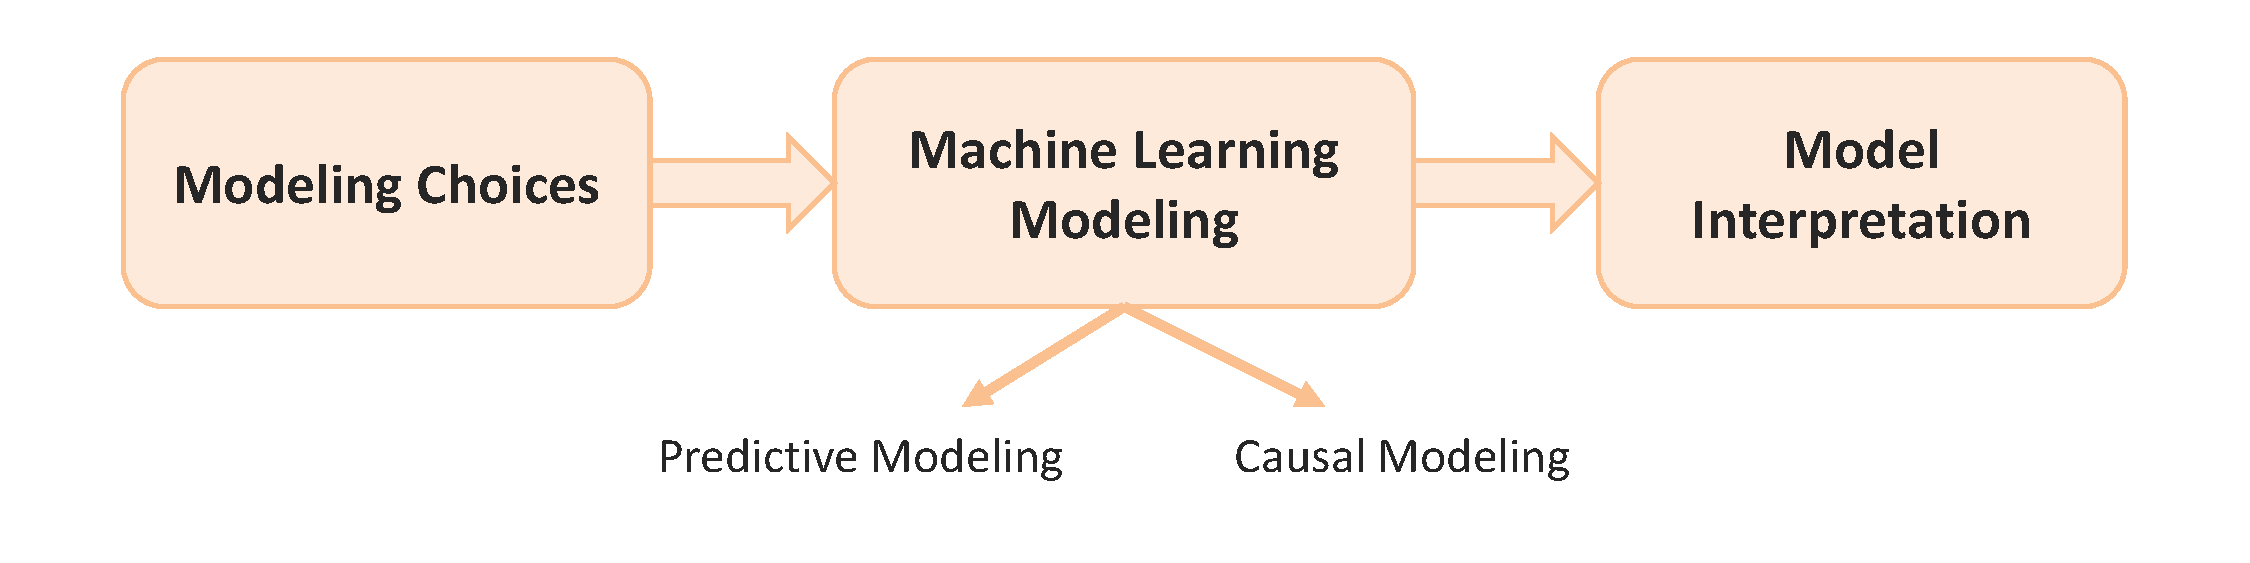
\includegraphics[width=6.5in]{ch1Fig1.pdf}
\caption{Illustration for the typical machine learning modeling pipeline.}
\end{figure}

\section{Machine Learning for Individualized Medicine}
% The typical pipeline

By machine learning (ML) we mean the process by which computer systems can learn directly from data, examples and experience, rather than being taught on the basis of predetermined rules. The purpose of this chapter is to illustrate some of the progress ML has already made in healthcare and to suggest some of the progress it might make --- and ought to make --- in the near future. The view presented here is deliberately optimistic; for ML to have a chance to achieve this potential --- as we believe it does --- there must first be a vision of what is possible. Topol has discussed at length the potential of accumulating more data; our focus here is on extracting more information from that data.

Our biggest challenge now is not whether we have enough data but whether we can combine the limitless potential of machines and the perennially limited potential of human judgement and decision making to use the oceans of data in which we are already swimming. And we should be careful to call out different dimensions of data. It covers electronic medical records, the collection and use of phenotypic and genetic data, data around performance and outcomes at an individual and population level and so on. And further, it will engage a wider range of data about the social determinants of health --- in areas like housing employment, retail patterns, income and inequality data --- whose impact on health intervention and outcomes will be increasingly critical. 

The rapid digitization of healthcare has led to a proliferation of clinical data, manifesting through electronic health records, biorepositories, and disease registries. This dissertation addresses the question of how machine learning (ML) techniques can capitalize on these data resources to assist clinicians in predicting, preventing and treating illness. To this end, we develop a set of ML-based, data-driven models of patient outcomes that we envision to be embedded within systems of decision support deployed at different stages of patient care.

We are in the midst of a revolution in the amount of data being generated. There are
many uses for this data; it can be analyzed and interpreted, often through powerful machine learning algorithms, edited, manipulated, distilled or reconstructed, and synchronized. In all cases the data must also be stored. All of these tasks must be performed in an environment of uncertainty; the underlying data operated on is never guaranteed to be reliable. The data may have been changed or edited knowingly or unknowingly, and is always subject to corruption from transmission and storage noise.

\subsection{Models for Cross-sectional Data}
\subsection{Models for Longitudinal Data}

\section{Outline of Contributions}
\subsection*{Chapter 2 Contributions}
\subsection*{Chapter 3 Contributions}
\subsection*{Chapter 4 Contributions}
\subsection*{Chapter 5 Contributions}
\subsection*{Chapter 6 Contributions}


\chapter{Estimating Treatment Effects from Observational Data}

For text, let's use the first words out of the ispell dictionary.

\chapter{Symbolic Approaches to Prognostic Model Interpretability}

\chapter{Automated Prognostic Modeling}

\chapter{Deep Probabilistic Modeling of Longitudinal Data}

For text, let's use the first words out of the ispell dictionary.

\chapter{Clinical Application}

\chapter{Conclusions}

\nocite{*}
\bibliographystyle {unsrt} %{thesis}
\bibliography {thesisrefs}    % bibliography references

\end {document}

